\documentclass[letterpaper, 11pt]{article} 

\usepackage{graphics,graphicx}
\usepackage{multicol} 
\usepackage{parskip}
\usepackage{amsmath}
\usepackage{multirow}
\usepackage[utf8]{inputenc}
\usepackage{fancyhdr}
\usepackage[title]{appendix}
\usepackage{wasysym}
\usepackage{url}
\usepackage{subcaption}

\usepackage[font=footnotesize,labelfont=small]{caption}
\captionsetup{width=0.85\linewidth}

\RequirePackage{geometry}
\geometry{margin=2cm}

\setlength{\parskip}{0.2cm}
\setlength{\parindent}{0pt}


\title{Assignment 1: Optics and Photoreceptors}
\author{
Tai Duc Nguyen \\
BMES T580: Systems Neuroscience in Medicine and Engineering
}
\date{\today}

\begin{document}

\maketitle

\rule{\textwidth}{1pt}

\section{Problem 1}
\label{sec:prob1}
\textbf{Problem statement:} Human eyes can resolve at a spatial frequency of 4175/rad (wow! We are good). When you go to an ophthalmologist to get an eye exam, you look at letters 20 feet away. What is the minimum spacing between lines that one can resolve if the lines are 20 feet away?

\textbf{Answer:}

\begin{figure}[htb!]
	\centering
	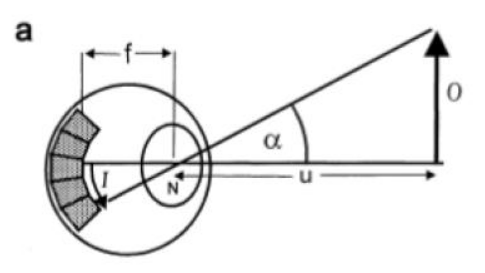
\includegraphics[width=0.6\linewidth]{1_fig.png}
%	\caption{DFF's Layout in Cadence's Virtuoso Layout Suite}
	\label{fig1}
\end{figure}

From the image above, it is easy to see the relationship of:
\begin{equation}
	\frac{I}{f} = \alpha = \frac{O}{U}
\end{equation}

And, the spatial frequency of the eye, in this case, is the same as its sampling frequency ($v_s$):
\begin{equation}
	v_s = \frac{f}{2I} = \frac{1}{2\alpha}
\end{equation}

Hence,

\begin{equation}
	v_s = \frac{U}{2O} = 4175 \text{ cycles/radians}
\end{equation}

\begin{equation}
	\frac{20 \text{ ft}}{2\times O} = 4175 \text{ cycles/radians}
\end{equation}

\begin{equation}
	O = \frac{20 \text{ ft}}{4175 \text{ cycles/radians} \times 2} = 0.00240 \text{ ft} = 0.73 \text{ mm}
\end{equation}

Therefore, the minimum spacing between lines that one can resolve at 20 feet away is about 0.73 millimeters.

\section{Problem 2}
\label{sec:prob2}
\textbf{Problem statement:} This eye has an aperture D = 3 mm and f = 4.2 mm. The diameter of the photoreceptor is 10 microns and the photoreceptors are closely packed.

a. What is the theoretical resolution of this eye?

b. What is the diffraction limit for this eye? If you get a different answer for the theoretical resolution than the diffraction, explain the possible reasons for the discrepancy?

c. The Modulation transfer function for this eye: $MTF(f) = e^{-24f^2}$. What is the cut-off spatial frequency for this eye?

d. Under a given light condition, there is N photons absorbed by the photoreceptors if the photoreceptors were receiving light from a white paper. What would be the cut-off frequency under these lighting conditions when this eye is looking at a scene with contrast = 1.

\textbf{Answer:}

a. As we have known, $v_s = \frac{f}{2I}$, hence, assuming that I (the diameter of the photoreceptors) is 10 $\mu m$, then:

\begin{equation}
	v_s = \frac{4.2 \times 10^{-3}}{2\times 10\times 10^{-6}} = 210 \text{ cycles/radians}
\end{equation}

b. The diffraction limit is given by:

\begin{equation}
	\omega = \frac{\lambda}{D} = \frac{0.5\times 10^{-6}}{3\times 10^{-3}} = 0.000167
\end{equation}

Hence, the resolution calculated from the diffraction limit is:

\begin{equation}
	R = \frac{1}{\omega} = \frac{1}{0.000167} = 6000 \text{ cycles/radians}
\end{equation}

Of course, 6000 cycles/radians is much larger than the theoretical 200 cycles/radians. The reason for this huge discrepancy relies on 2 parameters: 1) the focal length ($f$), and 2) the diameter of the photoreceptor ($I$). Since $f$ is short and $I$ is very larger, the ratio $\frac{f}{I}$ is much smaller than that of humans ($f = 17 \text{ mm}$ and $I = 2 \mu m$). 

c. The cut-off spatial frequency for this eye should be well approximated by its retinal sampling frequency ($v_s$). Hence:

\begin{equation}
	v_{co} = v_s = 210 \text{ cycles/radians}
\end{equation}

d. Since the eye is looking at the scene at the contrast = 1 (100\%), the cut-off frequency is still 210 cycles/radians.

\section{Problem 3}
\label{sec:prob3}
\textbf{Problem statement:} 
a. Which of the following is/are true for rod phototransduction?
\begin{enumerate}
	\item The membrane potential decreases in response to light.
	\item The concentration of calcium ions increases in response light.
	\item The concentration of cGMP decreases in response to light.
	\item The concentration of cAMP decreases in response to light.
\end{enumerate}
b. The traces below show the response of a rod photoreceptor to flashes to light. Brief(20 millisecond) flashes of light of increasing intensity produce increasing responses. Rmax is the maximum response. The traces shown here are normalized to that maximum response. Answer the following questions:
\begin{enumerate}
	\item What is the membrane potential of the rods at rest (i.e. in dark or before 0 seconds in this trace)? Briefly, explain your answer.
	\item Why does it take the response ~100 milliseconds to reach its peak when the flash is only 20 milliseconds long?
	\item You can see from the figure that as one increases the light level, the response does not increase. It saturates. Why does it saturate? As one increases the light level beyond the intensity needed to saturate the rods, the response stays saturated for longer. Why does the response stay saturated for longer?
\end{enumerate}

\begin{figure}[htb!]
	\centering
	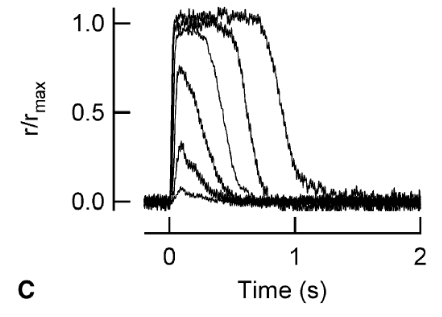
\includegraphics[width=0.6\linewidth]{2_fig.png}
	%	\caption{DFF's Layout in Cadence's Virtuoso Layout Suite}
	\label{fig2}
\end{figure}

\textbf{Answer:}

In response to light (photo absorbed by rhodopsin or iodopsin):
\begin{itemize}
	\item The Schiff base cofactor inside rhodopsin or iodopsin change from cis to trans creating transducin, which binds to a G protein in the membrane
	\item Each transducin will then activate the enzyme cGMP-specific PDE
	\item Each PDE then catalyzes the hydrolysis of cGMP to 5' GMP
	\item Hence, concentration of cGMP is reduced, causing closure of cyclic nucleotide-gated Na+ ion channels.
	\item As concentration of Na+ drops, the cell's membrane is hyperpolarized
	\item This negative change in membrane potential causes voltage-gated calcium channels to close, which reduces the concentration of Ca+ ions
	\item The reduction in Ca+ level causes the amount of the neurotransmitter glutamate to drop, which induces depolarization of on-center bipolar cells and hyperpolarization of cone off-center bipolar cells
\end{itemize}

a. Hence, 1 and 3 is correct, while 2 and 4 is not. cAMP is not mentioned in the process above due to the fact that it "has been believed to play an important role in the organization of circadian rhythms in the vertebrate eye but not to be directly involved in controlling the phototransduction cascade in photoreceptors...Changes in cAMP levels have regulatory influences on the photoreceptor cascade...increasing [photoreceptors'] sensitivity during the dark part of the day and decreasing its sensitivity in bright light." \textit{Astakhova, L.A., Kapitskii, S.V., Govardovskii, V.I. et al. Cyclic AMP as a Regulator of the Phototransduction Cascade. Neurosci Behav Physi 44, 664–671 (2014). https://doi.org/10.1007/s11055-014-9967-5}

1b. Since the graph is normalized, it is not possible to guess the membrane potential of the rods at rest ($R/R_{max} = 0$). However, this number is often assumed to be around -40mV

2b. The event of a photon getting absorbed by rhodopsin or iodopsin happens almost instantaneous; however, the cascading result of it requires a lot more time: the catalyzation of cGMP to 5'GMP causing the cascading closure of Na+ channels, which then cause the Ca+ channels to close.

3b. The response does not increase after it reaches $R_{max}$ is because there are a finite number of Na+ and Ca+ channels. When all of them closes and the level of Na+/Ca+ is stabilized, then there is no more change in membrane potential. 

Also, increasing the light intensity should cause a phenomenon called "bleaching". The more intense the light, the more photons which can react with rhodopsin and cause the high level depletion of this protein. Hence, it takes more time to convert the rhodopsins back the more rhodopsins getting depleted.

\section{Problem 4}
\label{sec:prob4}
\textbf{Problem statement:} 

a. What is the receptive field of a photoreceptor?

b. RGC has a center-surround receptive field. What is a center-surround receptive field?

c. The figure below shows an example of a recording from primate retina. Answer the following questions about the recording below:
\begin{enumerate}
	\item Just by looking at the recording, you can make a pretty firm conclusion about the cell type being recorded. Make the conclusion and explain why?
	\item Based on the recording below, please draw/describe the receptive field of this cell.
\end{enumerate}

\begin{figure}[htb!]
	\centering
	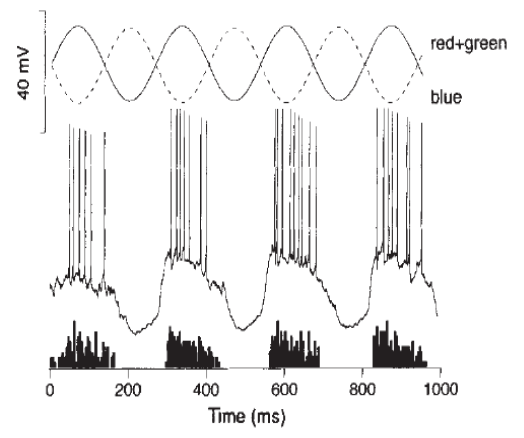
\includegraphics[width=0.7\linewidth]{3_fig.png}
	%	\caption{DFF's Layout in Cadence's Virtuoso Layout Suite}
	\label{fig3}
\end{figure}

\textbf{Answer:}

a. The receptive field of a single photoreceptor cell corresponds to this photoreceptor's precise location on the retina.

b. There are two types of bipolar cells, distinguished by the way they respond to light on the centers of their receptive fields. They are called ON-center cells and OFF-center cells. ON-center cells depolarized when light hit the center, OFF-center cells depolarized when light hit the surround.

1c. From the recording, it looks like: 1) the cell depolarizes when expose to a red+green, and 2) hyperpolarizes when expose to blue. Hence, this is a yellow-ON, blue-OFF cell. 

2c. A yellow-ON, blue-OFF cell will have yellow in the center and blue in the surround if the cell is a ON-center cell. On the other hand, if the cell is a OFF-center cell, then blue will be in the middle and yellow will be on the surround.


%\begin{equation}
%Q=\begin{cases}
%1, & \text{Data if rising edge of Clock}.\\
%0, & \text{else keep previous data}
%\end{cases}
%\end{equation}

%\begin{figure}[htb!]
%	\centering
%	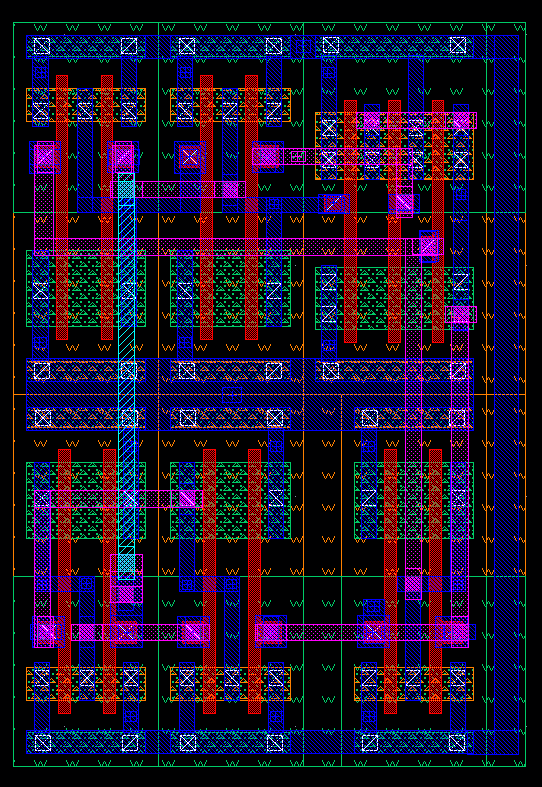
\includegraphics[width=0.6\linewidth]{dff_layout.png}
%	\caption{DFF's Layout in Cadence's Virtuoso Layout Suite}
%	\label{fig8}
%\end{figure}


%\begin{figure}[ht!]
%	\centering
%	\begin{subfigure}[b]{.48\linewidth}
%		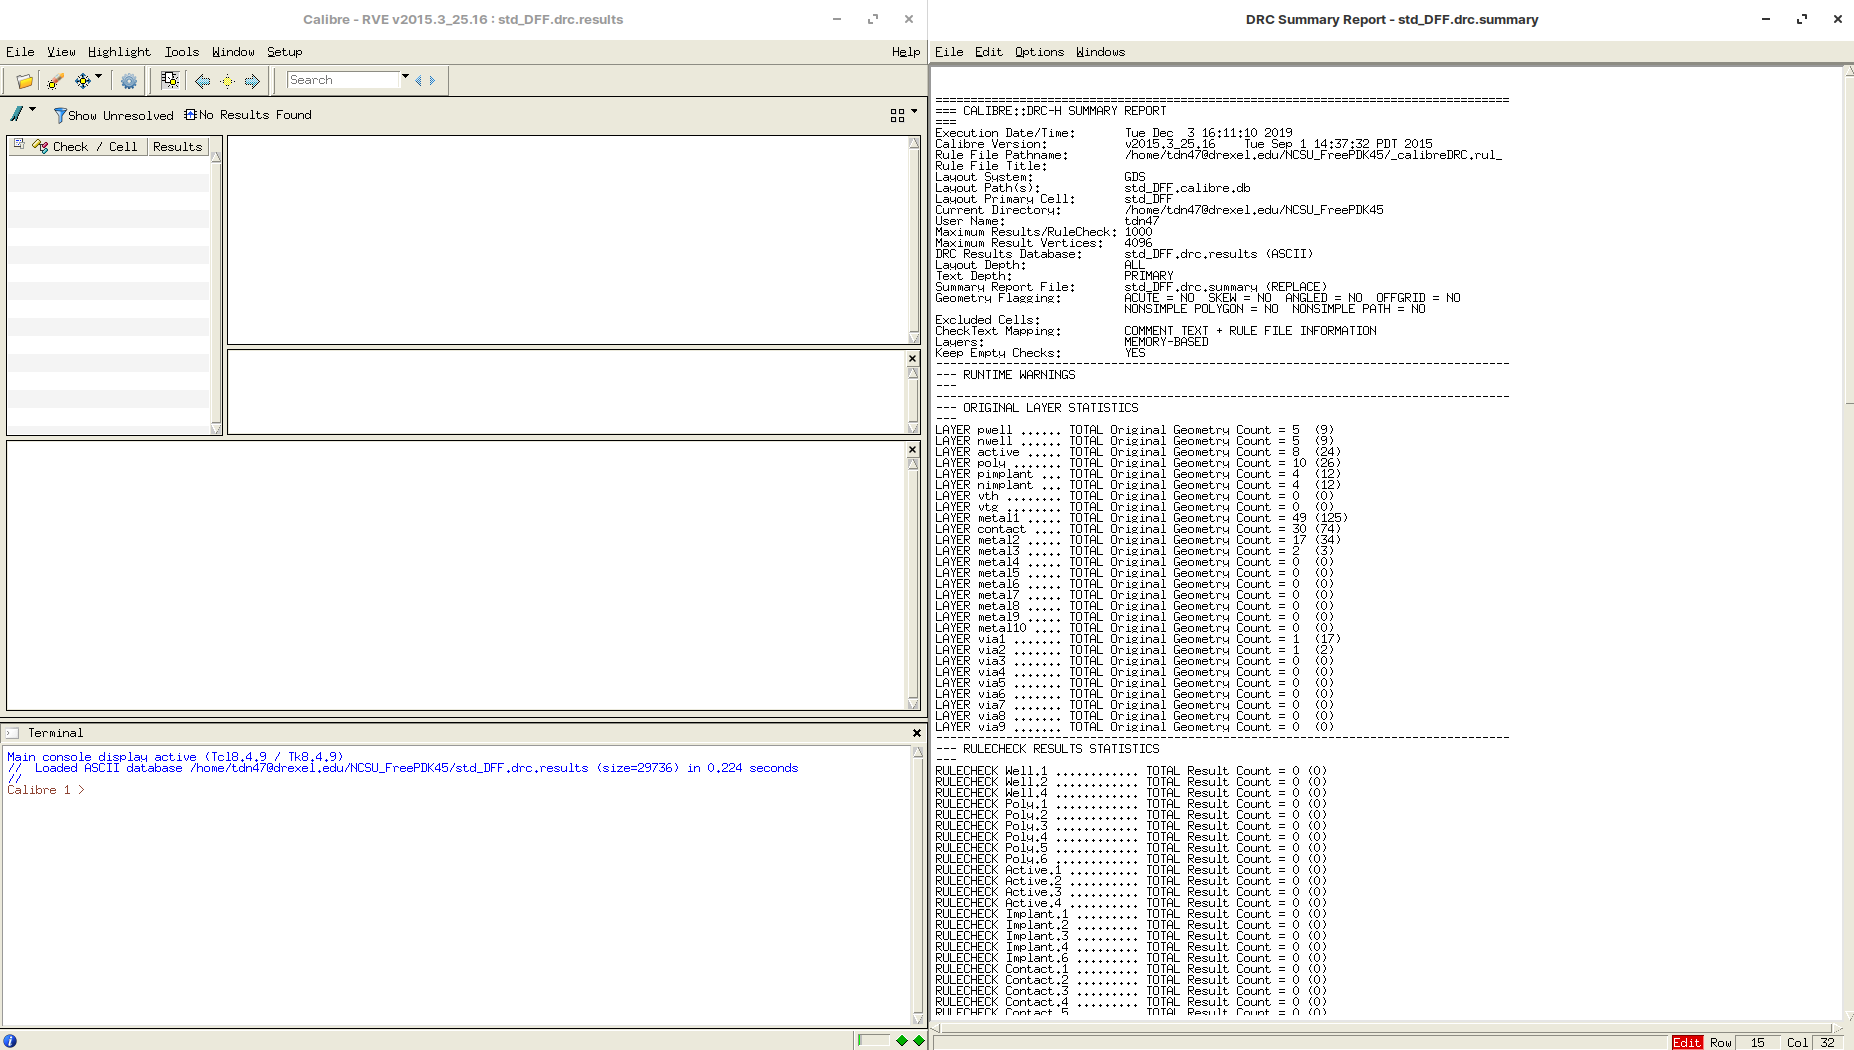
\includegraphics[width=\textwidth]{dff_drc.png}
%		\caption{DFF's rise and fall time}
%		\label{fig9a}
%	\end{subfigure}
%	%	\hskip2em
%	\begin{subfigure}[b]{.48\linewidth}
%		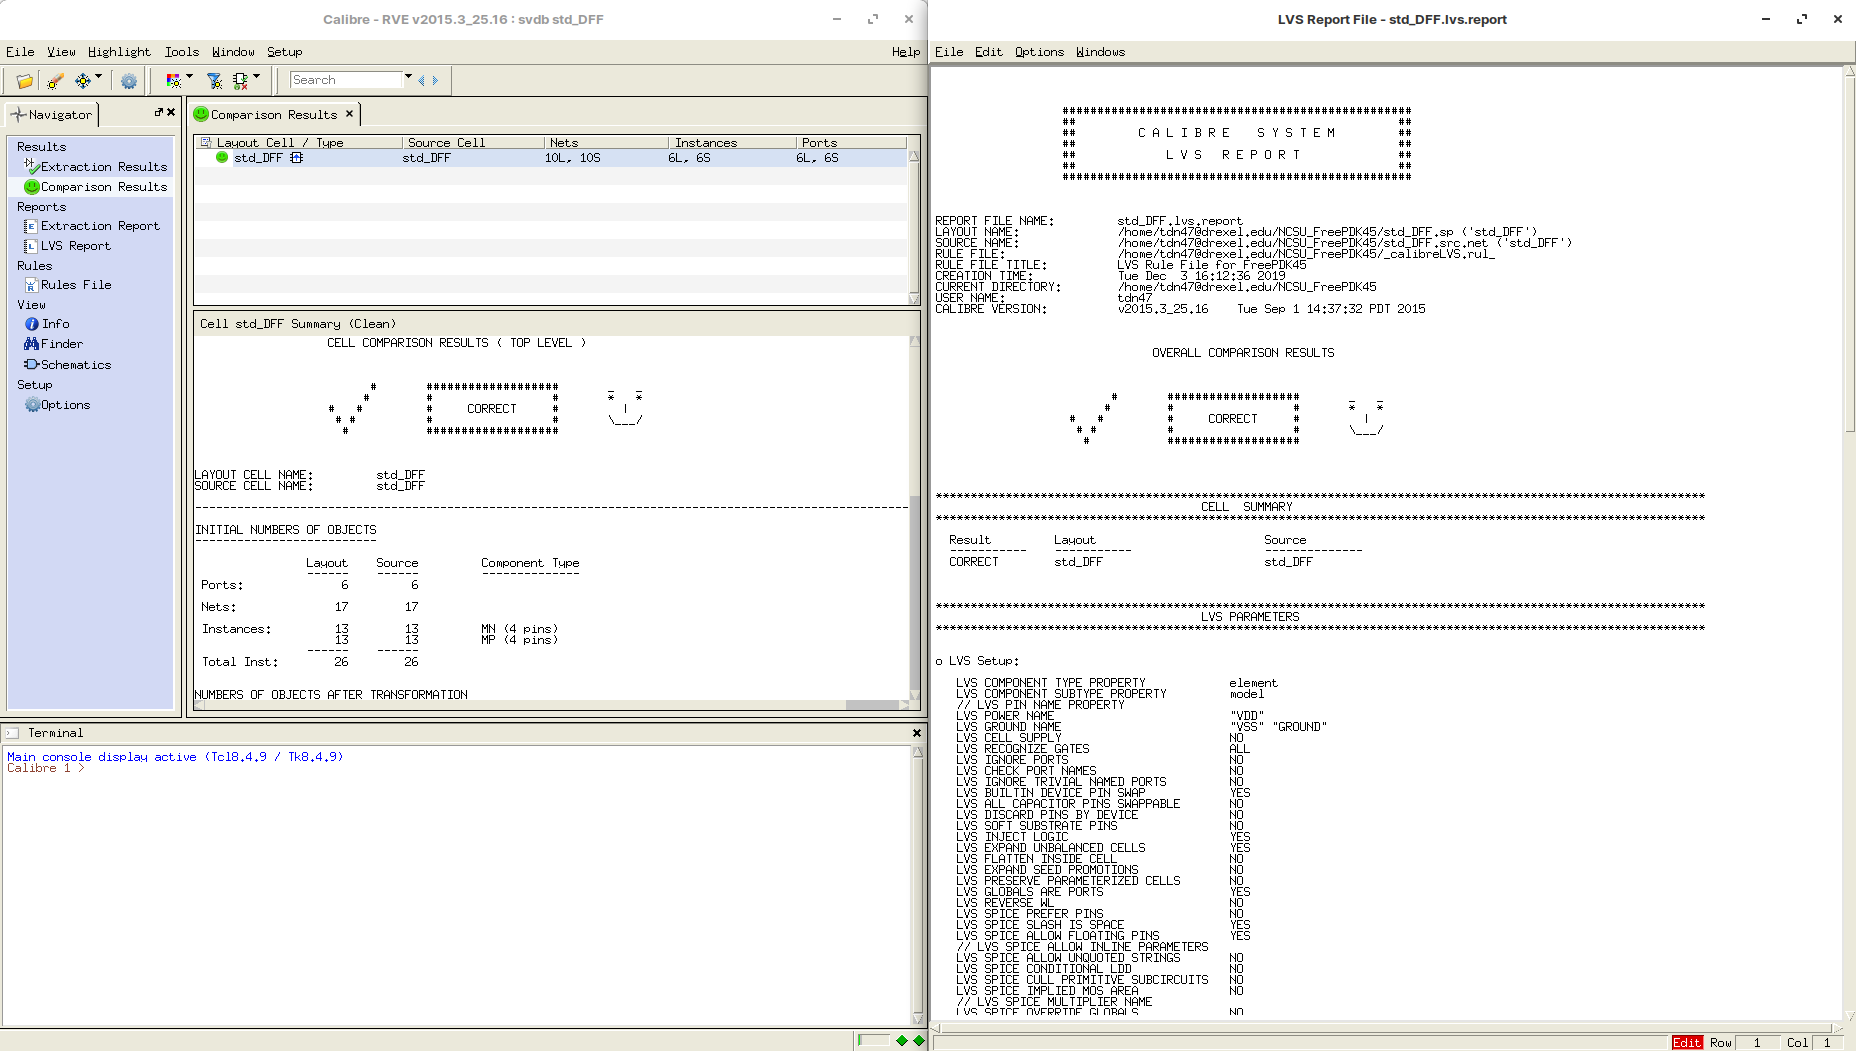
\includegraphics[width=\textwidth]{dff_lvs.png}
%		\caption{DFF's propagation delay}
%		\label{fig9b}
%	\end{subfigure}
%	\caption{Measurements of the DFF's rise/fall time and propagation delay}
%\end{figure}

\end{document}